\section*{Βήμα 7.1}
\subsection*{Ερώτημα α}
Ξεκινάμε παραθέτοντας την καμπύλη του training loss για το CNN που εκπαιδεύεται στο MNIST. 

\begin{figure}[H]
	\centering
	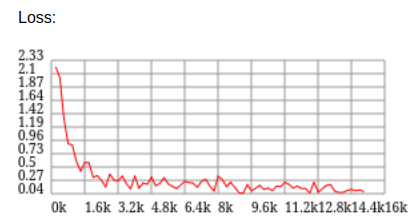
\includegraphics[width=0.8\linewidth]{images/step7a_training_loss.png}
\end{figure}

\noindent Βλέπουμε ότι πρακτικά το loss έχει πάψει να μειώνεται, επομένως το μοντέλο έχει φτάσει το όριο των δυνατοτήτων του. \\

\noindent \textbf{Επίπεδο εισόδου:} \\

\noindent Στο πρώτο αυτό layer, ουσιαστικά έχουμε την εικόνα μεγέθους 24x24. Τα gradient έχουν πλέον μικρύνει τόσο πολύ διότι το μοντέλο έχει ήδη συγκλίνει, όπως βλέπουμε και στο γράφημα παραπάνω. Οι διορθώσεις είναι πλέον αμελητέες, ειδικά σε αυτό το επίπεδο που είναι το πιο βαθύ κατά το back propagation.

\begin{figure}[H]
	\centering
	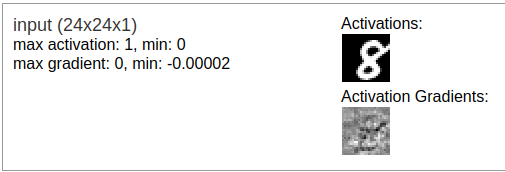
\includegraphics[width=0.9\linewidth]{images/step7a_input.png}
\end{figure}

\noindent \textbf{Πρώτο συνελικτικό επίπεδο:} 

\begin{figure}[H]
	\centering
	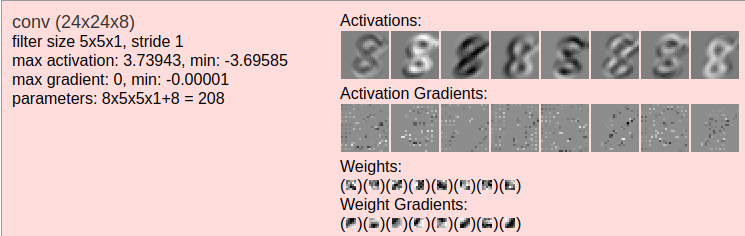
\includegraphics[width=0.9\linewidth]{images/step7a_conv1.png}
\end{figure}

\noindent Αυτό το επίπεδο χρησιμοποιεί 8 κανάλια με kernels διάστασης 5x5. Βλέποντας τα activations, βλέπουμε ότι σχηματίζονται ανάγλυφα των ψηφίων. Τα gradients, συσσωρεύονται γύρω από το περίγραμμα των ψηφίων. Αυτό μας ωθεί να συμπεράνουμε ότι πρόκειται για έναν ανιχνευτή ακμών ή γωνιών. Γενικά χαρακτηριστικών που οφείλονται σε χρωματικές αντιθέσεις. Πρακτικά, αυτό το επίπεδο εξάγει τα θεμελιώδη γεωμετρικά χαρακτηριστικά των ψηφίων. Τα gradients είναι μικρά για τον ίδιο λόγο με πριν. \\

\noindent \textbf{ReLU:} \\

\begin{figure}[H]
	\centering
	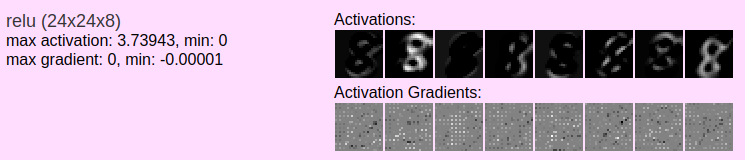
\includegraphics[width=0.9\linewidth]{images/step7a_relu.png}
\end{figure}

\noindent Ο ρόλος της ReLU είναι αφενός να εισάγει μη-γραμμικότητα στο μοντέλο αυξάνοντας τη χωρητικότητά του, καθιστώντας το ικανό να περιγράψει πιο περίπλοκες εξαρτήσεις και αφετέρου να καταστέλει το overfitting κρατώντας μόνο τα θετικά activations. \\

\noindent \textbf{Pooling:}

\noindent Το pooling μειώνει την χωρική διάσταση των χαρακτηριστικών επιλέγοντας τη μεγαλύτερη τιμή από ένα ορισμένο παράθυρο από pixels. Αυτό το layer συμβάλλει καθοριστικά στην βασική ιδιότητα των CNN, το translation invariance και λειτουργεί σαν κάποιας μορφής regularization. Η οπτικοποίηση που μας δίνεται από την ιστοσελίδα φαίνεται παρακάτω:

\begin{figure}[H]
	\centering
	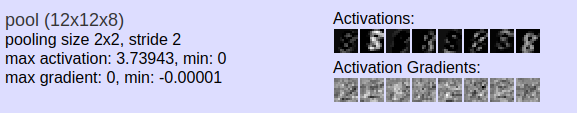
\includegraphics[width=0.9\linewidth]{images/step7a_pooling.png}
\end{figure}

\noindent \textbf{Δεύτερο συνελικτικό επίπεδο}

\begin{figure}[H]
	\centering
	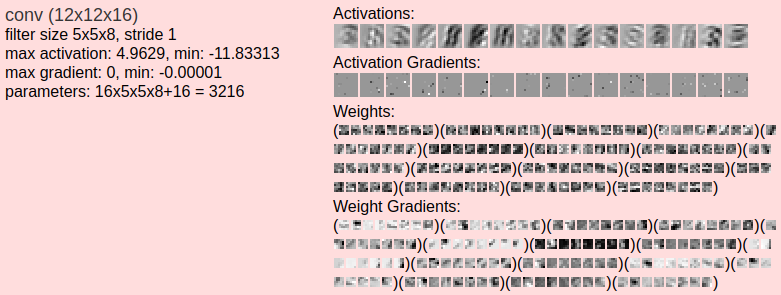
\includegraphics[width=0.9\linewidth]{images/step7a_conv2.png}
\end{figure}

\noindent Το δεύτερο συνελικτικό επίπεδο του δικτύου έχει πιο αφηρημένες ενεργοποιήσεις και gradients. Έτσι, αντιλαμβανόμαστε πως έχει να κάνει με συγκεκριμένα μοτίβα κάθε ψηφίου, όπως τους κύκλους στο 8 που βλέπουμε στην εικόνα μας. Τα κανάλια που χρησιμοποιούνται εδώ είναι 16, περισσότερα από πριν. Αυτό είναι λογικό αφού το πλήθος των αφηρημένων χαρακτηριστικών που θα θέλαμε να αναγνωρίσουμε στα ψηφία μας είναι σχετικά μεγαλύτερος από τα πρωτογενή τους γεωμετρικά χαρακτηριστικά (γραμμές και κύκλοι). \\

\noindent Ακολουθούν ένα επίπεδο ReLU και Pooling όπως και πριν με ακριβώς τις ίδιες λειτουργίες. 

\begin{figure}[H]
	\centering
	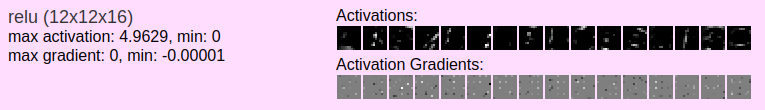
\includegraphics[width=0.9\linewidth]{images/step7a_relu2.png}
\end{figure}

\begin{figure}[H]
	\centering
	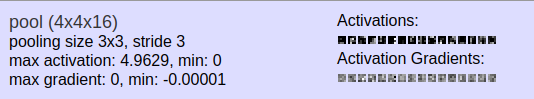
\includegraphics[width=0.9\linewidth]{images/step7a_pool2.png}
\end{figure}

\noindent \textbf{Fully Connected Επίπεδο:}

\noindent Το επίπεδο αυτό αναλαμβάνει την τελική ταξινόμηση. Επειδή είναι fully connected συνδυάζει όλη την πληροφορία και τα features που έχουν εξαχθεί από τα συνελικτικά επίπεδα που προηγήθηκαν και καταλήγει σε ένα μονοδιάστατο διάνυσμα με μήκος 10 (μία θέση για κάθε ψηφίο).

 \begin{figure}[H]
 	\centering
 	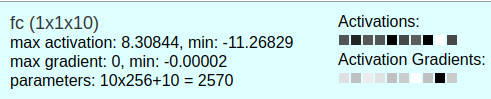
\includegraphics[width=0.9\linewidth]{images/step7a_fc.png}
 \end{figure}
 
 \noindent Προφανώς και η πιο σκούρη-έντονη ενεργοποίηση αντιστοιχεί στο προτελευταίο ψηφίο, δηλαδή το 8 που είναι και αυτό που εξετάζουμε. \\
 
 \noindent \textbf{Softmax:}
 
  \begin{figure}[H]
 	\centering
 	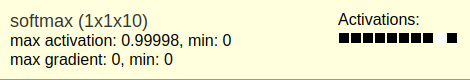
\includegraphics[width=0.9\linewidth]{images/step7a_softmax.png}
 \end{figure}
 
 \noindent Το τελευταίο αυτό επίπεδο κανονικοποιεί την έξοδο του fully connected layer στο διάστημα (0, 1) επιτρέποντάς μας να ερμηνεύσουμε την τελική έξοδο ως πιθανότητα για την αναγνώριση του εκάστοτε ψηφίου. 
 
 \subsection*{Ερώτημα β}
 
 Η υλοποίησή μας βασίζεται στο backbone του εργαστηρίου και φαίνεται παρακάτω:
 
  \begin{figure}[H]
 	\centering
 	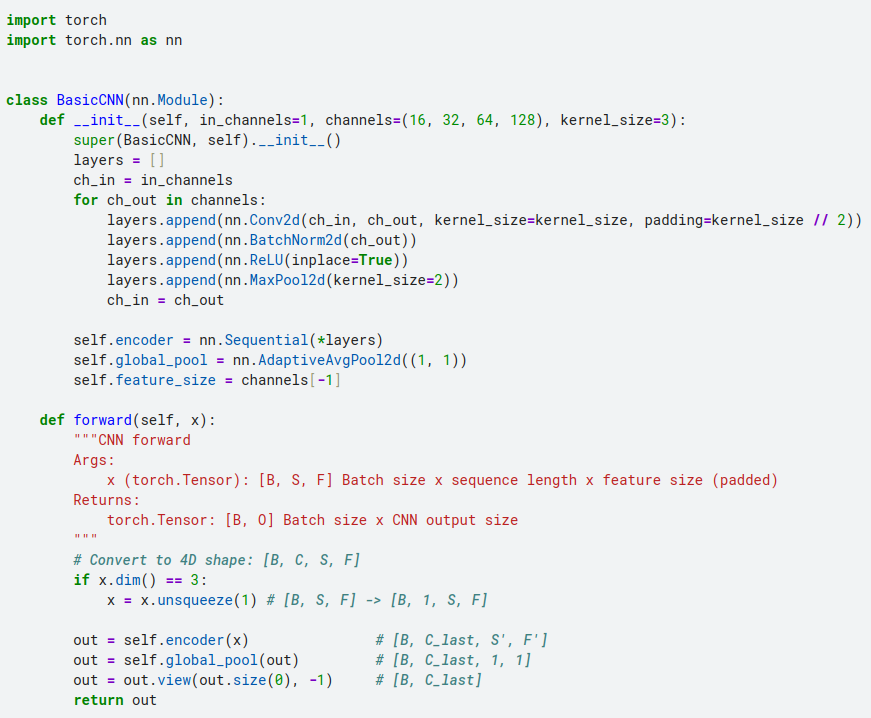
\includegraphics[width=0.9\linewidth]{images/step7b_cnn.png}
 \end{figure}
 
 \noindent Ακολουθώντας τις επιταγές της εκφώνησης χρησιμοποιούμε τα ζητούμενα layers και στη συνάρτηση forward κάνουμε τους υπολογισμούς τους διαδοχικά τον έναν μετά τον άλλο. Θα πραγματοποιήσουμε και θα σχολιάσουμε την εκπαίδευση στο ερώτημα δ.
 
 \subsection*{Ερώτημα γ}
 
 \textbf{Convolutions:} Ο ρόλος των συνελίξεων είναι να εφαρμόζουν ένα φίλτρο στην είσοδο και έτσι να υπολογίζουν ένα feature map του. Τα φίλτρα δεν είναι τίποτα άλλο από kernels με tunable βάρη τα οποία αποτελούν τις παραμέτρους του δικτύου. Είναι ο λόγος που λέμε ότι το CNN χαρακτηρίζεται από parameter sharing. Το feature map υπολογίζεται με το εσωτερικό γινόμενο της εισόδου με τον kernel. \\
 
 \noindent \textbf{Batch Normalization:} Ο ρόλος του Batch Normalization είναι να κανονικοποιεί τα activations κάθε batch επιβάλλοντάς τους να ακολουθούν κανονική κατανομή με μηδενική μέση τιμή και μοναδιαία διασπορά. Αυτό ομαλοποιεί την συνάρτηση κόστους, επιταχύνει την εκπαίδευση και λειτουργεί ως regularizer. Συνήθως εφαρμόζεται μεταξύ της εξόδου ενός συνελικτικού επιπέδου και της ReLU (ή άλλης συνάρτησης ενεργοποίησης). \\
 
 \noindent \textbf{ReLU:} Η ReLU αυξάνει τη χωρητικότητα του μοντέλου εισάγοντας μια μη γραμμικότητα σε αυτό. Έτσι του επιτρέπει να μαθαίνει πιο περίπλοκες εξαρτήσεις και μοτίβα στα δεδομένα. Επιπλέον καταστέλει τις αρνητικές ενεργοποιήσεις, κάνοντας το σύνολό τους πιο αραιό. \\
 
 \noindent \textbf{Max Pooling:} Ουσιαστικά υποδειγματολειπτεί την είσοδο επιλέγοντας τη μεγαλύτερη τιμή που υπάρχει κάθε φορά μέσα στο παράθυρο που καλύπτει ο kernel. Έτσι, αφενός μειώνει τη διαστατικότητα της εισόδου απλοποιώντας τους υπολογισμούς και αφετέρου συμβάλλει στο translation invariance των CNN. 
 
 \subsection*{Ερώτημα δ}
 
 Εκτελούμε την εκπαίδευση του CNN στη λειτουργία overfit batch και παίρνουμε τα εξής:
 
 \begin{figure}[H]
 	\centering
 	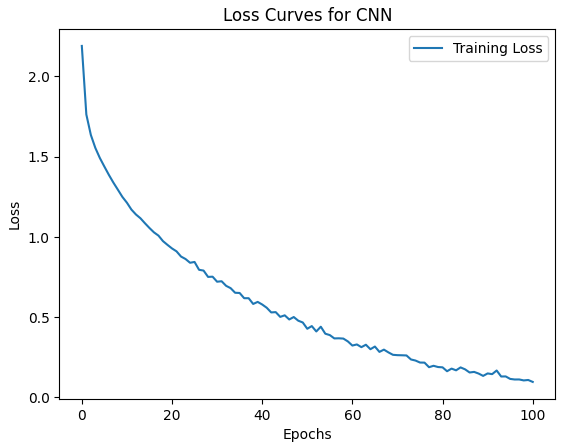
\includegraphics[width=0.75\linewidth]{images/step71d_loss.png}
 \end{figure}
 
 \begin{figure}[H]
	\centering
	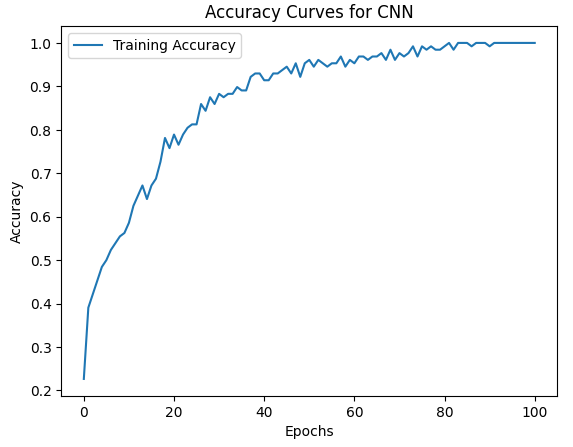
\includegraphics[width=0.75\linewidth]{images/step71d_acc.png}
\end{figure}

\noindent Το δίκτυο υπερπροσαρμόστηκε στην εποχή 101. Αυτό σημαίνει ότι πράγματι είναι ικανό να μάθει τα μοτίβα για το task μας. 
 
\subsection*{Ερώτημα ε}
Το kernel που επιλέγουμε έχει μέγεθος 3x3. Εκπαιδεύουμε το μοντέλο μας και παίρνουμε τα εξής:

 \begin{figure}[H]
	\centering
	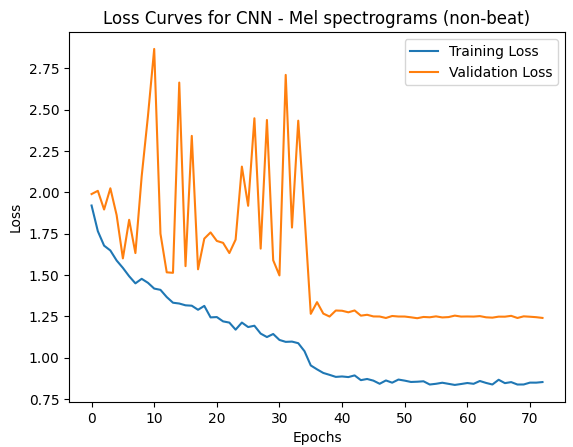
\includegraphics[width=0.75\linewidth]{images/step71e_loss.png}
\end{figure}

\begin{figure}[H]
	\centering
	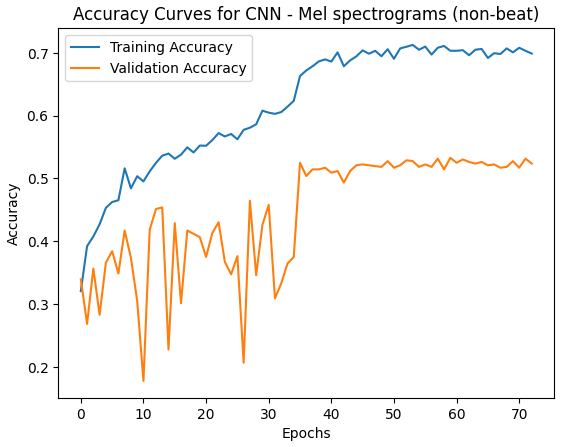
\includegraphics[width=0.75\linewidth]{images/step71e_acc.png}
\end{figure}

\noindent Το μοντέλο τα πηγαίνει καλύτερα από το LSTM της προπαρασκεύης αφού πετυχαίνει καλύτερα σκορ τόσο στα δεδομένα εκπαίδευσης όσο και στα δεδομένα επικύρωσης. Παρόλα αυτά το θέμα με την αδυναμία γενίκευσης δεν έχει επιλυθεί. Τα χαρακτηριστικά που εξάγουν τα feature maps του CNN είναι μεν καλύτερα αλλά ούτε αυτά επαρκούν για την επίτευξη μεγάλων επιδόσεων στο task. \\

\noindent Μερικά στατιστικά συνοψίζονται παρακάτω:

\begin{figure}[H]
	\centering
	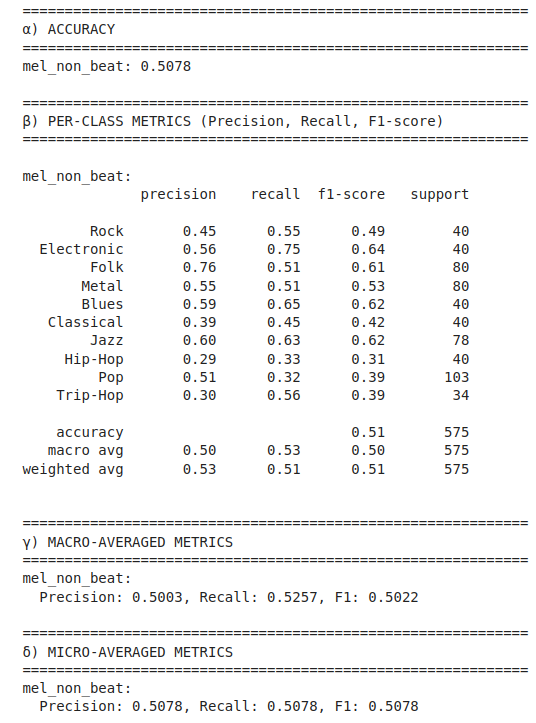
\includegraphics[width=0.5\linewidth]{images/step71e_statistics.png}
\end{figure}

\section*{Βήμα 7.2}

\subsection*{Ερώτημα α}
Η λειτουργία του μοντέλου περιγράφεται συνοπτικά στα παρακάτω βήματα:

\begin{itemize}
	\item Είσοδος και Δημιουργία Φασματογραφήματος: Το αρχικό ηχητικό σήμα μετατρέπεται σε μια ακολουθία χαρακτηριστικών (log Mel filterbank), δημιουργώντας ένα 2D φασματογράφημα (spectrogram).

	\item Διαχωρισμός σε Τμήματα (Patch Splitting): Το φασματογράφημα χωρίζεται σε μια ακολουθία από τετράγωνα τμήματα (patches) μεγέθους 16×16, τα οποία έχουν επικάλυψη (overlap) μεταξύ τους.

	\item Γραμμική Προβολή και Embeddings: Κάθε τμήμα (16×16) ισοπεδώνεται (flatten) και προβάλλεται σε ένα μονοδιάστατο διάνυσμα (patch embedding) μέσω ενός γραμμικού επιπέδου.

	\item Πληροφορία Θέσης (Positional Embedding): Επειδή ο Transformer δεν αντιλαμβάνεται εγγενώς τη σειρά εισόδου, προστίθεται σε κάθε patch embedding μια εκπαιδεύσιμη πληροφορία θέσης, ώστε το μοντέλο να μπορεί να συλλάβει τη χωρική δομή του 2D φασματογραφήματος.

	\item Επεξεργασία μέσω Transformer: Στην αρχή της ακολουθίας προστίθεται ένα ειδικό διακριτικό ταξινόμησης ([CLS] token). Η συνολική ακολουθία εισάγεται στον Κωδικοποιητή του Transformer (Transformer Encoder), ο οποίος χρησιμοποιεί την τυπική αρχιτεκτονική χωρίς τροποποιήσεις.

	\item Ταξινόμηση: Η έξοδος του Transformer που αντιστοιχεί στο [CLS] token χρησιμοποιείται ως η αναπαράσταση του ηχητικού φασματογραφήματος. Ένα τελικό γραμμικό επίπεδο με σιγμοειδή ενεργοποίηση μετατρέπει αυτή την αναπαράσταση σε ετικέτες για την ταξινόμηση.
\end{itemize}

\subsection*{Ερώτημα β}
Χρησιμοποιώντας την υλοποίηση του εργαστηρίου εκπαιδεύουμε το ast χρησιμοποιώντας το base384. Τα αποτελέσματα της εκπαίδευσης παρουσιάζονται παρακάτω:

\begin{figure}[H]
	\centering
	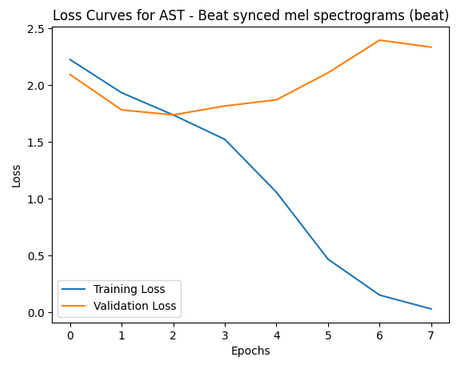
\includegraphics[width=0.5\linewidth]{images/step72_loss.png}
\end{figure}

\begin{figure}[H]
	\centering
	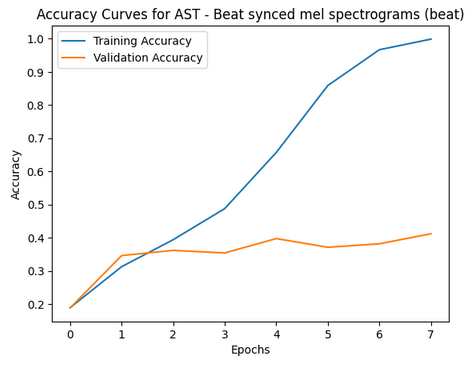
\includegraphics[width=0.5\linewidth]{images/step72_acc.png}
\end{figure}

\noindent Βλέπουμε μία textbook περίπτωση overfit. Το validation accuracy αγγίζει το 1 ενώ το loss τείνει στο 0. Ταυτόχρονα, η απόδοση στο validation dataset είναι πάρα πολύ κακή. Αυτό σημαίνει ότι η χωρητικότητα του transformer είναι πάρα πολύ μεγάλη με αποτέλεσμα σε ελάχιστες εποχές (7) να αποστηθίζει τα δεδομένα εκπαίδευσης. Για να το αντιμετωπίσουμε θεωρητικά θα χρειαζόμασταν είτε πολύ μεγαλύερο όγκο δεδομένων είτε πολύ έντονο regularization. 

\section*{Βήμα 8}
\subsection*{Ερώτημα α}
Τα μοντέλα των προηγούμενων ερωτημάτων εκτελούσαν την ταξινόμηση αξιοποιώντας ένα fully connected layer στο τέλος τους. Έτσι, η έξοδός τους, έπαιρνε μία από τις 10 διακριτές τιμές που αντιστοιχούν στις κλάσεις του προβλήματός μας. 

\noindent Στο πρόβλημα της παλινδόμησης, όμως, δε θέλουμε τα μοντέλα μας να παίρνουν διακριτές τιμές, αλλά συνεχείς. Έτσι αλλάζουμε το fully connected layer και επιβάλουμε 1 έξοδο. Αυτή παίρνει συνεχείς τιμές, το output του νευρώνα. \\

\noindent Επιπλέον, μετρικές όπως το accuracy, precision, recall και f1 score δεν έχουν νόημα στο πλαίσιο της παλινδρόμησης. Για αυτό αφενός αντικαθιστούμε το CrossEntropy με το MSELoss και αφετέρου υπολογίζουμε την ίδια συνάρτηση τόσο στο train όσο και στο validation set ώστε να αξιολογήσουμε το μοντέλο μας. \\

\noindent Ο κώδικας που ορίζει τα μοντέλα μας με τις αλλαγές που περιγράψαμε φαίνεται παρακάτω:

\begin{figure}[H]
	\centering
	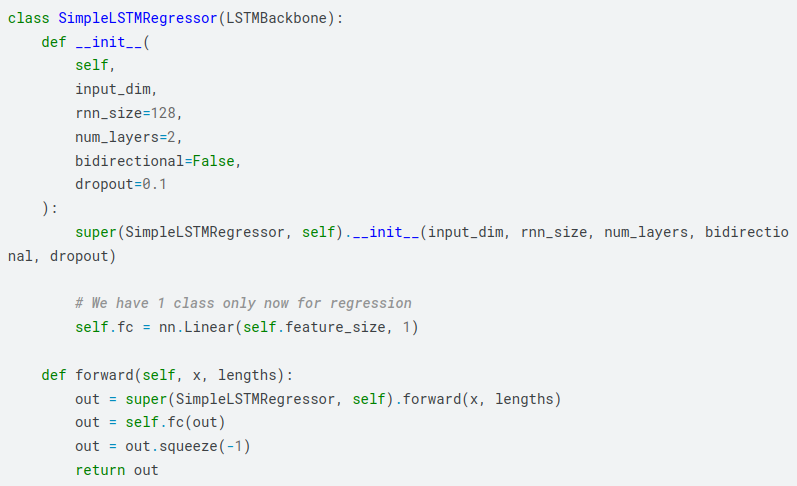
\includegraphics[width=0.8\linewidth]{images/lstm_regressor.png}
\end{figure}

\begin{figure}[H]
	\centering
	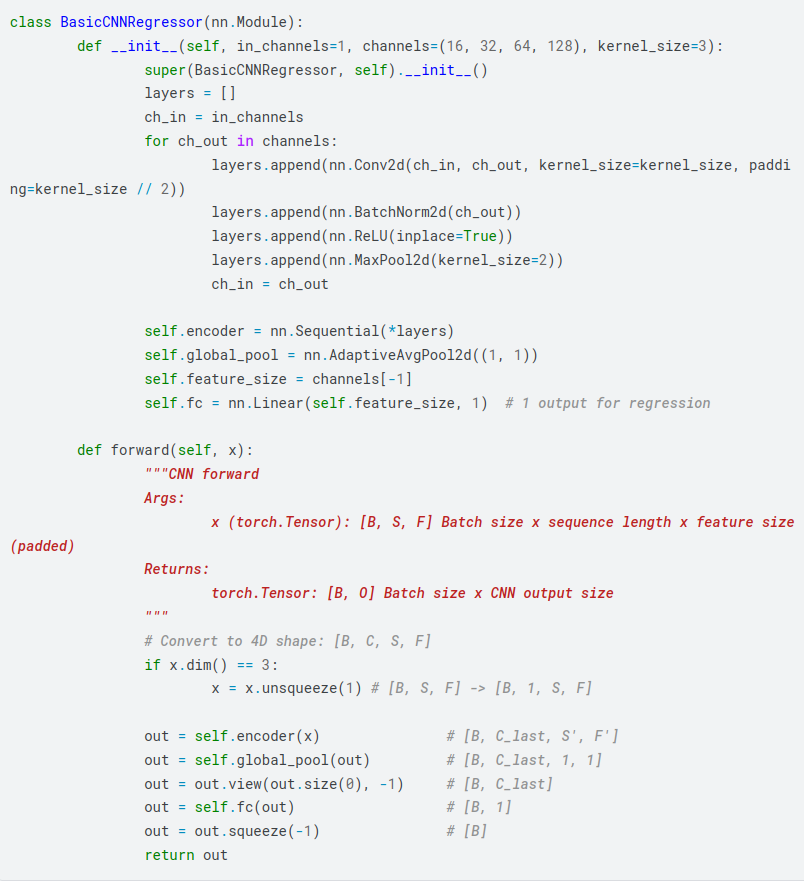
\includegraphics[width=0.7\linewidth]{images/cnn_regressor.png}
\end{figure}

\subsection*{Ερώτημα β}

Αρχικά, φτιάχνουμε τους dataloaders που θα χρησιμοποιήσουμε για την εκπαίδευση των μοντέλων στο task μας. 

\begin{figure}[H]
	\centering
	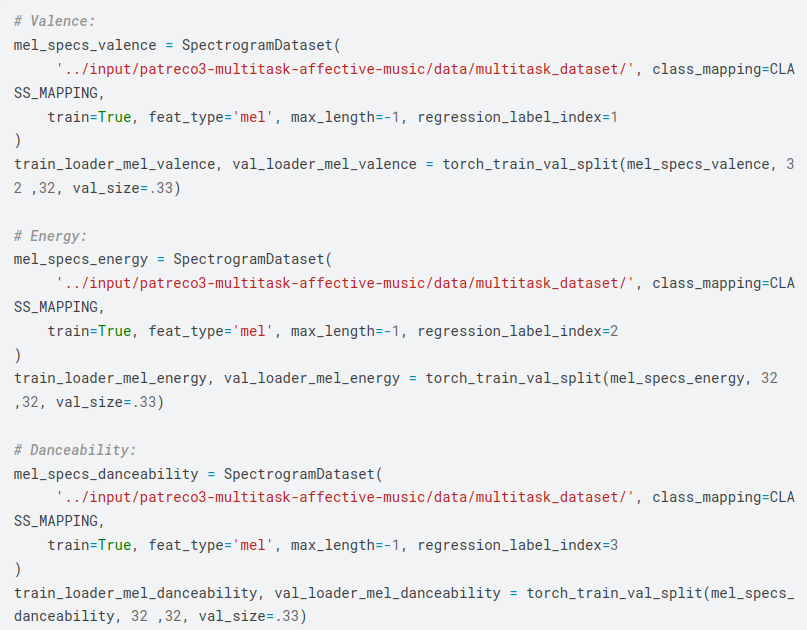
\includegraphics[width=0.7\linewidth]{images/step8b_dataloaders.png}
\end{figure}

\noindent Όπως φαίνεται παραπάνω, χρησιμοποιούμε τις βοηθητικές συναρτήσεις το κώδικα του εργαστηρίου αλλάζοντας το directory των δεδομένων και επισημαίνοντας το label το οποίο επιθυμούμε να εξετάσουμε (regression\_label\_index). \\

\noindent Εκπαιδεύουμε τα μοντέλα μας για το valence. Ξεκινάμε με το LSTM. 

\begin{figure}[H]
	\centering
	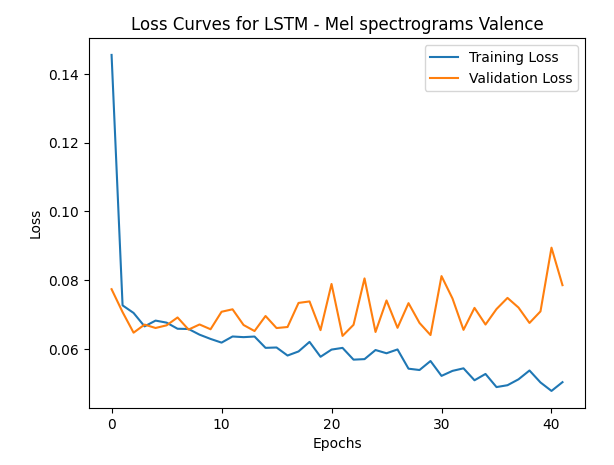
\includegraphics[width=0.7\linewidth]{images/step8b_lstm_valence.png}
\end{figure}

Ακολουθεί η εκπαίδευση του CNN:

\begin{figure}[H]
	\centering
	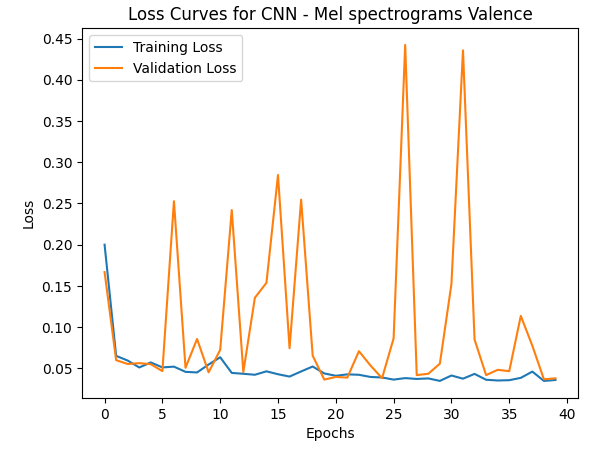
\includegraphics[width=0.7\linewidth]{images/step8b_cnn_valence.png}
\end{figure}

\noindent Τα 2 μοντέλα πετυχαίνουν τελικά αρκετά καλό τελικό MSE τόσο στο training set όσο και στο validation set. Ελαφρώς καλύτερα τα πηγαίνει το CNN, στο οποίο μάλιστα δεν εμφανίζεται (τουλάχιστον τόσο έντονα) η απουσία ικανότητας γενίκευσης, παρότι γενικά το validation loss είναι πιο ασταθές. 

\subsection*{Ερώτημα γ}

Ακολουθεί η εκπαίδευση των μοντέλων για την κατηγορία energy.

\begin{figure}[H]
	\centering
	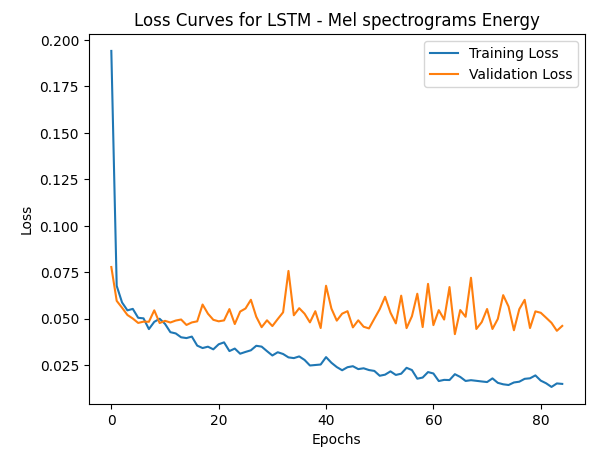
\includegraphics[width=0.8\linewidth]{images/step8c_lstm_energy.png}
\end{figure}

\begin{figure}[H]
	\centering
	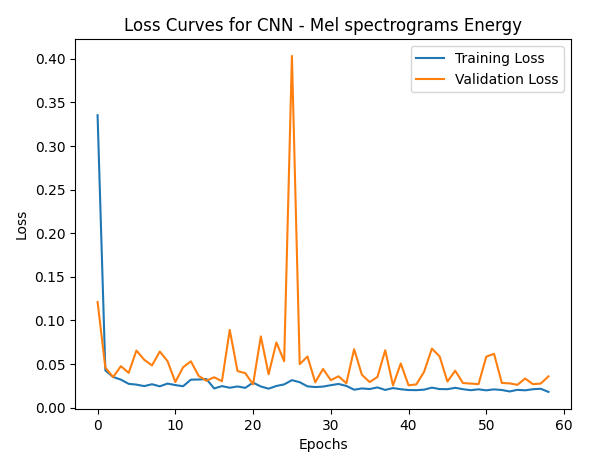
\includegraphics[width=0.8\linewidth]{images/step8c_cnn_energy.png}
\end{figure}

\noindent Σε αυτό το task και τα 2 μοντέλα τα πηγαίνουν καλύτερα από το προηγούμενο. Συγκεκριμένα το CNN ρίχνει το MSE κάτω από 0.01 πετυχαίνοντας πολύ καλή επίδοση. Αυτή τη φορά πρακτικά το CNN επιδεικνύει ικανότητες γενίκευσης σε αντίθεση με το LSTM που παραμένει πιο αδύναμο σε αυτό τον τομέα. Επιπλέον το CNN συγκλίνει και σε λιγότερες εποχές από το LSTM.

\subsection*{Ερώτημα δ}

Ακολουθούν τα αποτελέσματα της εκπαίδευσης των μοντέλων για το task του danceability. 

\begin{figure}[H]
	\centering
	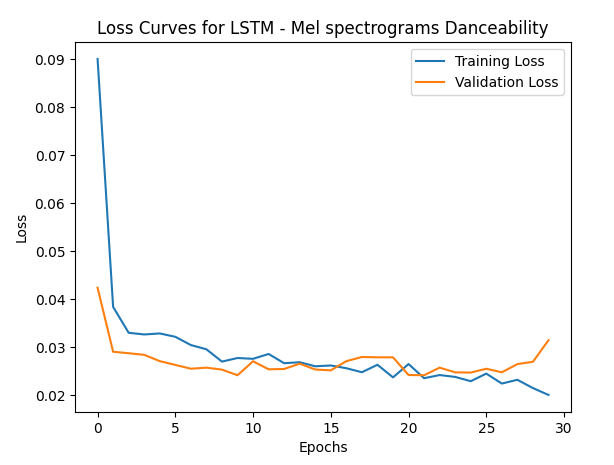
\includegraphics[width=0.7\linewidth]{images/step8d_lstm_dance.png}
\end{figure}

\begin{figure}[H]
	\centering
	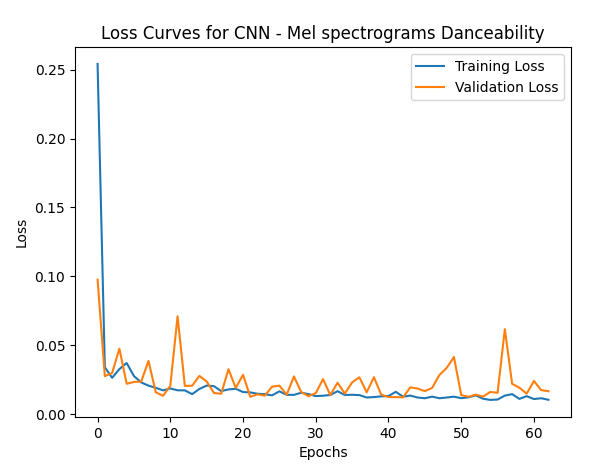
\includegraphics[width=0.7\linewidth]{images/step8d_cnn_dance.png}
\end{figure}

\noindent Για ακόμα μία φορά και τα 2 μοντέλα τα πηγαίνουν καλά σε αυτό το task έχοντας MSE τάξης μεγέθους $10^{-2}$ με το CNN πάλι να πετυχαίνει την καλύτερη επίδοση. Σε αντίθεση με τα προηγούμενα tasks, το LSTM εμφανίζεται να γενικεύει ικανοποιητικότερα ενώ συγκλίνει και γρηγορότερα σε σχέση με το CNN.

\subsection*{Ερώτημα ε}

Το Spearman correlation είναι ένας αριθμός στο (-1, 1) που δείχνει πόσο συσχετισμένα είναι 2 σύνολα από ranks. Δεν χρειάζεται η συσχέτιση των 2 αυτών συνόλων να είναι γραμμική, το spearman correlation δουλεύει και για μη γραμμικές συσχετίσεις. \\

\noindent Τα spearman correlation για τα μοντέλα μας παρουσιάζονται παρακάτω:

\lstinputlisting{documents/spearman.txt}

\noindent Το μεγαλύτερο spearman correlation το πετυχαίνουμε για το CNN. 

\section*{Βήμα 9}
\subsection*{Ερώτημα α}
Στο paper της αναφοράς [5] εξετάστηκαν βαθιά συνελικτικά δίκτυα ως προς τη γενικότητα ή την εξειδίκευση των νευρώνων τους και συνεπώς τη δυνατότητά τους να μεταφέρουν χρήσιμη γνώση-χαρακτηριστικά με transfer learning. Τα συμπεράσματά του μπορούν να συνοψιστούν με 2 προτάσεις:

\begin{enumerate}
	\item Το transferability γνώσης επηρεάζεται αρνητικά από εξειδικευμένους νευρώνες στα υψηλότερα στρώματα του δικτύου και από co-adapted νευρώνες στο μέσο τους.
	
	\item Ακόμα και αν το original task απέχει αρκετά από το target task, η αρχικοποίηση του δικτύου με transferred features προωθεί καλύτερα το generalization μετά από fine tuning σε σχέση με τη αρχικοποίηση με τυχαία features.   
\end{enumerate} 

\subsection*{Ερώτημα β}
Επιλέγουμε το μοντέλο του 7.1, δηλαδή το CNN. Στα προηγούμενα task είχε καλύτερη απόδοση από το LSTM, ενώ παραμένει σχετικά ελαφρύ και εκπαιδεύεται γρηγορότερα από όλα. 

\subsection*{Ερώτημα γ}

Εκπαιδεύουμε το CNN στο fused dataset, γιατί είναι το πιο πλούσιο σε πληροφορία, οπότε θα επιτρέψει στο CNN να εξάγει τις καλύτερες αναπαραστάσεις. Το καλύτερο μοντέλο αποθηκεύεται στο checkpoint, γίνεται restored στο τέλος της εκπαίδευσης και αποθηκεύεται στο trained\_cnn['fused\_non\_beat']

\noindent ['model']. Η μετρική που διαλέγουμε για την αξιολόγηση είναι το MSELoss. Επιπλέον, προφανώς θα δώσουμε μεγαλύτερη βαρύτητα στο αποτέλεσμα στο validation set αφού αυτό θα μας βοηθήσει να αντιληφθούμε φαινόμενα υπερπροσαρμογής ή στην ικανότητα γενίκευσης του μοντέλου. \\

\noindent Εκπαιδεύουμε το μοντέλο μας και παρουσιάζουμε τα αποτελέσματα:

\begin{figure}[H]
	\centering
	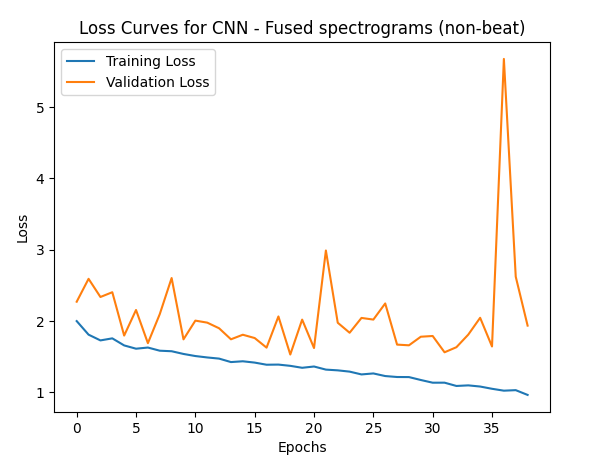
\includegraphics[width=0.7\linewidth]{images/step9c_loss.png}
\end{figure}

\noindent Ακολουθεί το αντίστοιχο διάγραμμα για το accuracy:

\begin{figure}[H]
	\centering
	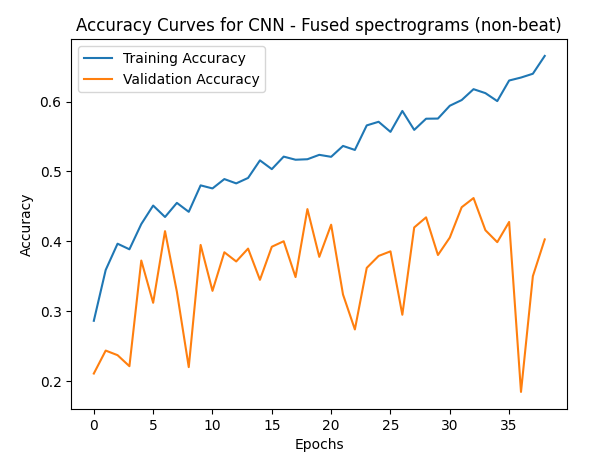
\includegraphics[width=0.7\linewidth]{images/step9c_acc.png}
\end{figure}

\noindent Βλέπουμε ότι τα αποτελέσματα του μοντέλου στο validation set είναι γενικά θορυβώδη ενώ μπορεί κανείς να διακρίνει και υπερπροσαρμογή του μοντέλου, αφού το τελικό validation accuracy απέχει αρκετά στο training και το validation set. 

\subsection*{Ερώτημα δ}

Φτιάχνουμε adapter στο προηγούμενο μοντέλο, παίρνοντας τα βάρη του σε όλα εκτός από το τελευταίο επίπεδο και βάζοντας ως τελευταίο επίπεδο ένα fully connected Linear layer για το task του regression στο danceability.

\begin{figure}[H]
	\centering
	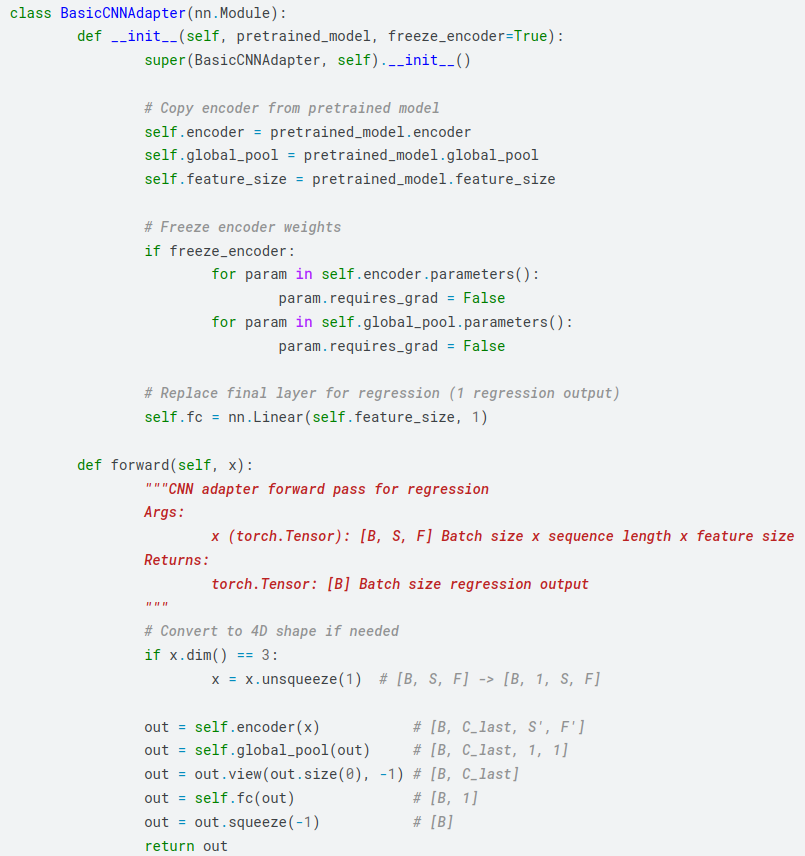
\includegraphics[width=0.6\linewidth]{images/step9d_adapter.png}
\end{figure}

\noindent Εκπαιδεύουμε τον adapter χρησιμοποιώντας το προεκπαιδευμένο CNN από το προηγούμενο ερώτημα:

\begin{figure}[H]
	\centering
	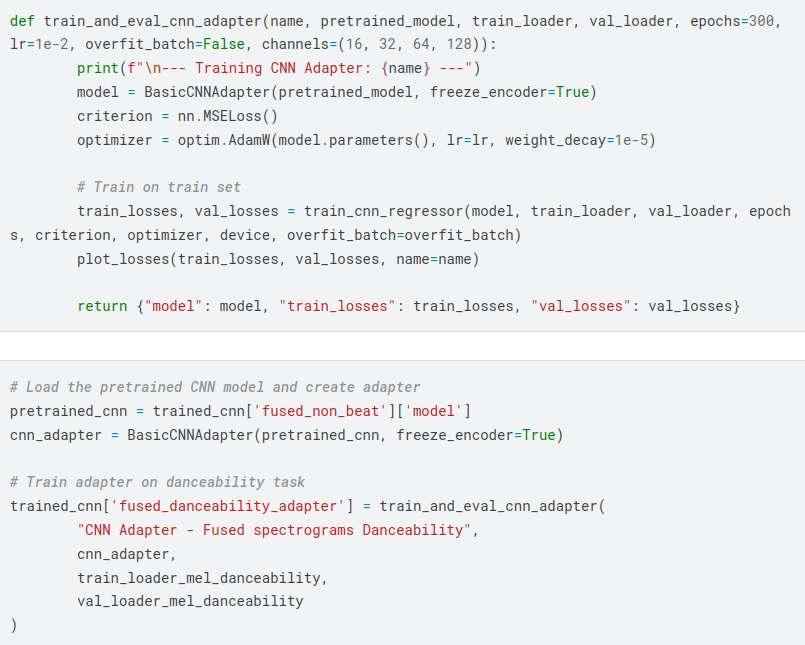
\includegraphics[width=0.7\linewidth]{images/step9d_train_eval.png}
\end{figure}

\noindent Το αποτέλεσμα φαίνεται παρακάτω:

\begin{figure}[H]
	\centering
	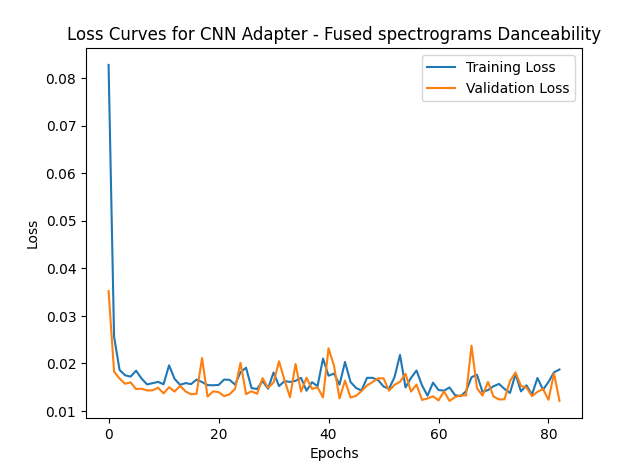
\includegraphics[width=0.7\linewidth]{images/step9d_adapter_res.png}
\end{figure}

\noindent Η βελτίωση είναι θεαματική. Όχι μόνο έχουμε καλύτερες μετρικές στο training και (κυρίως) στο validation set αλλά έχουμε εξομαλύνει και την εκπαίδευση του μοντέλου καθολικά. \\

\noindent Το αποτέλεσμα αυτό επιβεβαιώνει πειραματικά τα ευρύματα του paper που υποστηρίζουν ότι η αρχικοποίηση των features με εκείνα ενός προεκπαιδευμένου μοντέλου δίνει μεγάλο boost στη δυνατότητα γενίκευσης το μοντέλου μας

\subsection*{Ερώτημα ε}

Το αποτέλεσμά μας είναι πολύ καλύτερο σε σύγκριση με αυτό του βήματος 8. Αρχικά, παίρνουμε 4 φορές μικρότερο MSE από ότι στο αντίστοιχο task του βήματος 8. Επιπλέον, η εκπαίδευση είναι πολύ λιγότερο θορυβώδης ενώ δεν εμφανίζονται καθόλου σημάδια υπερπροσαρμογή ή απουσίας ικανότητας γενίκευσης. Όλα αυτά γίνονται με κόστος μόλις 20 περίπου εποχές εκπαίδευσης παραπάνω, αμελητέο σε σχέση με τα οφέλη που αποκομίζουμε από το transfer learning.

\section*{Βήμα 10}

\subsection*{Ερώτημα α}
Τα συμπεράσματα του paper της αναφοράς [7] με 2 προτάσεις είναι:

\begin{enumerate}
	\item Για πρώτη φορά αναπτύχθηκε ένα MultiModel βαθιάς μάθησης ικανό να μάθει ταυτόχρονα πολλαπλά tasks από διαφορετικούς τομείς και να έχει καλή απόδοση σε όλα τους.
	
	\item Ο τρόπος να το πετύχει κανείς αυτό είναι η χρήση πολλαπλών υπολογιστικών block με διαφορετική εξειδίκευση (convolution layers, attention mechanisms, encoders, decoders, ...) έτσι ώστε η εκπαίδευσή τους με όσες περισσότερες παραμέτρους μπορεί να αξιοποιήσει το transfer learning μεταξύ τους, ακόμα και αν τα δεδομένα δεν είναι πάρα πολλά. 
\end{enumerate}

\subsection*{Ερώτημα β}

Η συνάρτηση κόστους που θα χρησιμοποιήσουμε είναι το άθροισμα των MSE σε κάθε task. Δεν βάζουμε βάρος σε κανένα από αυτά αφού θέλουμε να τα πάμε εξίσου καλά σε κάθε task. 

\begin{figure}[H]
	\centering
	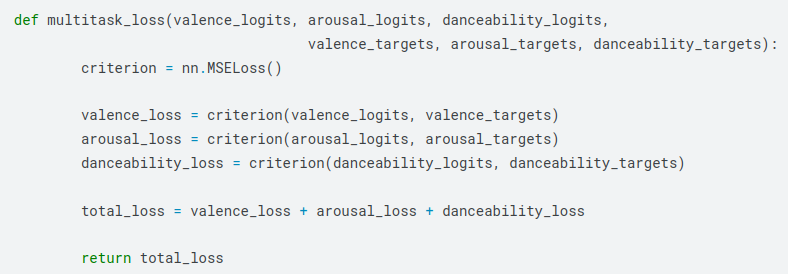
\includegraphics[width=0.8\linewidth]{images/step10b.png}
\end{figure}

\subsection*{Ερώτημα γ}

Αρχικά φτιάχνουμε dataloaders για το κάθε task χρησιμοποιώντας τα φασματογραφήματα mel.

\begin{figure}[H]
	\centering
	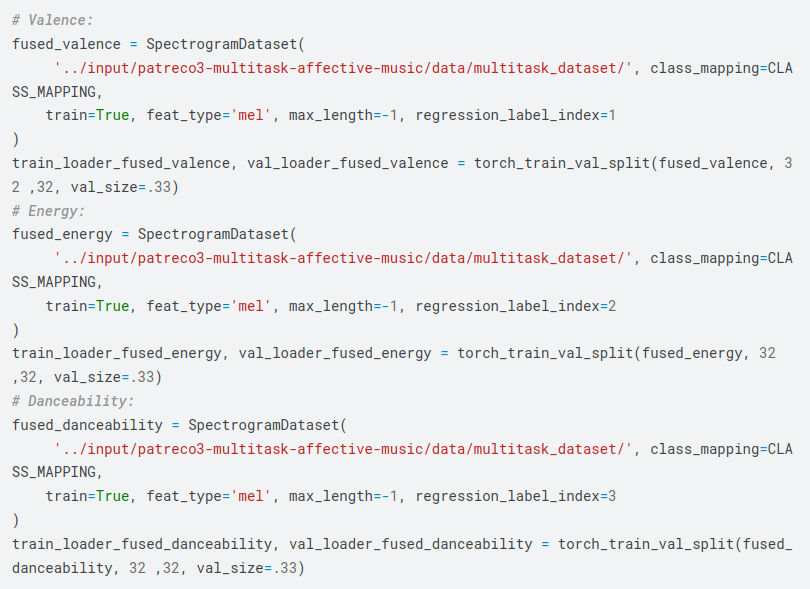
\includegraphics[width=0.8\linewidth]{images/step10d_dataloader.png}
\end{figure}

\noindent Στη συνέχεια όπως θα δείτε στο notebook που θα ανεβάσουμε ορίζουμε τον αντίστοιχο multiclass adapter και τον εκπαιδεύουμε χρησιμοποιώντας το προεκπαιδευμένο CNN. Το αποτέλεσμα φαίνεται στην επόμενη σελίδα. \\

\noindent Το αποτέλεσμα είναι εντυπωσιακό. Το άθροισμα των 3 losses είναι μικρότερο από 0.1 στο καλύτερο μοντέλο ενώ δεν φαίνονται σημάδια υπερπροσαρμογής ή απουσίας γενίκευσης. Όλα αυτά μόνο σε 16 εποχές! \\

\noindent Το παραπάνω αποτέλεσμα επιβεβαιώνει για ακόμα μια φορά τη δύναμη του transfer learning αλλά και το ότι η εκπαίδευση ενός μοντέλου για πολλά task είναι εφικτή.

\begin{figure}[H]
	\centering
	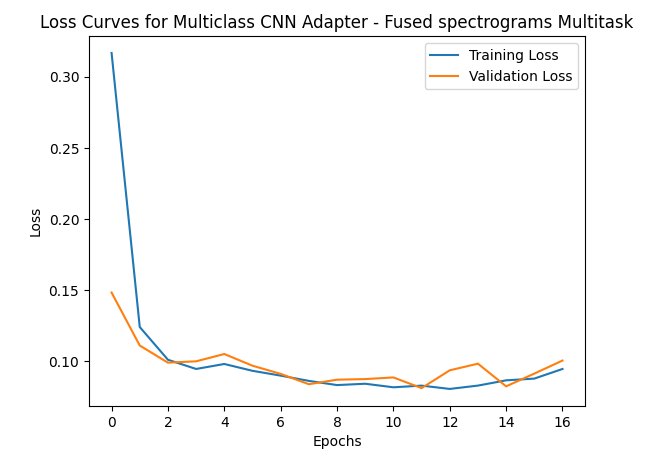
\includegraphics[width=0.8\linewidth]{images/step10_res.png}
\end{figure}

\noindent Παρακάτω παρουσιάζουμε και το spearman correlation για τα 3 tasks:

\begin{figure}[H]
	\centering
	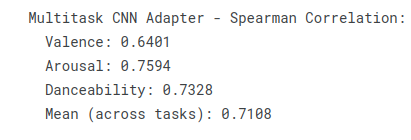
\includegraphics[width=0.8\linewidth]{images/step10_spearman.png}
\end{figure}

\noindent Τα αποτελέσματα είναι πολύ κοντά σε αυτά που πετύχαμε individually με μοντέλα και στα 3 tasks. Αυτό συμφωνεί με τα αποτελέσματα του paper [7].
